\section{Vektoren}
\subsection{Definition von Vektoren}
\begin{defi}{Vektoren}{}\index{Vektoren!Definition}
Die Menge aller parallelen, gleich langen und gleich gerichteten Pfeile nennt man Vektor. Jeder Pfeil ist der Repräsentant des Vektors.
\begin{center}

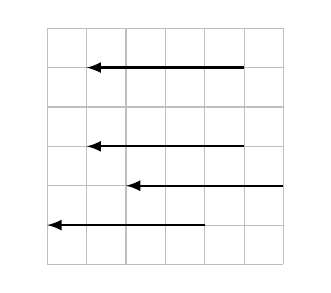
\begin{tikzpicture}[x=.5cm, y=.5cm,domain=-9:9,smooth, cross/.style={draw, cross out,
  minimum size=2*(#1-1pt), inner sep=0pt, outer sep=0pt},>=latex, font= \footnotesize]
   %Raster zeichnen
   \draw [color=gray!50]  [step=5mm] (-1,-1) grid (5,5);

\coordinate(a) at (4,4);
\coordinate(b) at (0,4);

\coordinate(c) at (4,2);
\coordinate(d) at (0,2);

\coordinate(e) at (5,1);
\coordinate(f) at (1,1);

\coordinate(g) at (3,0);
\coordinate(h) at (-1,0);
%Vektor
\draw[thick, ->] (a) node[right]{} -- (b) node[left]{};
\draw[thick, ->] (c) node[right]{} -- (d) node[left]{};
\draw[thick, ->] (e) node[right]{} -- (f) node[left]{};
\draw[thick, ->] (g) node[right]{} -- (h) node[left]{};
\end{tikzpicture}
\end{center}
Alle drei Pfeile sind Repräsentanten des selben Vektors.
\end{defi}
\begin{merke}{Bezeichnungen}{}\index{Vektoren!Bezeichnung}
Vektoren werden mit kleinen lateinischen Buchstaben und einem pfeil gekennzeichnet $\vec{u}$. Verläuft ein Repräsentant eines Vektors von einem Punkt z.B. $P$ zu einem zweiten Punkt z.B. $Q$, so bezeichnet man alle Repräsentanten mit $\vv{PQ}$.
\begin{center}

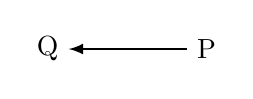
\begin{tikzpicture}[x=.5cm, y=.5cm,domain=-9:9,smooth, cross/.style={draw, cross out,
  minimum size=2*(#1-1pt), inner sep=0pt, outer sep=0pt},>=latex, ]
   %Raster zeichnen
% \draw [color=gray!50]  [step=5mm] (0,0) grid (3,3);
\coordinate(a) at (3,3);
\coordinate(b) at (0,3);
%Vektor
\draw[thick, ->] (a) node[right]{P} -- (b) node[left]{Q};
\end{tikzpicture}
\end{center}
\end{merke}
\begin{satz}{Vektoraddition}{}\phantomsection\label{vekadd}\index{Vektoren!Addition}
Bei der Addition von zwei Vektoren wird an den Endpunkt eines Repräsentanten des ersten Vektors $\vv{a}$ der Beginn eines Repräsentanten des zweiten Vektors $\vv{b}$ gesetzt. Der Pfeil des Summenvektors $\vv{c} = \vv{a} + \vv{b}$ ergibt sich durch den Pfeil der am Anfangspunkt des Vektors $\vv{a}$ beginnt und am Endpunkt des Vektors $\vv{b}$ endet.\\
Da es für einen Vektor unendlich viele Repräsentanten gibt, gibt es immer einen, der an der \glqq richtigen\grqq{} Stelle für eine Addition liegt.
\begin{center}
 
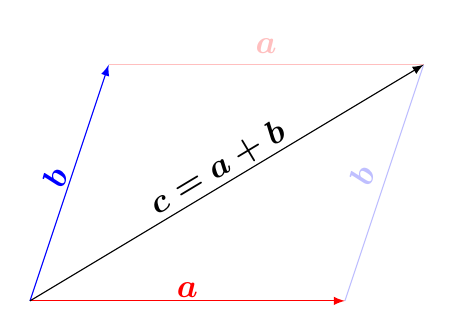
\begin{tikzpicture}[font=\boldmath]\large
    % Punkte
    \coordinate (A) at (0,0) {};
    \coordinate (B) at (4,0) {};
    \coordinate (C) at (1,3) {};
    \coordinate (D) at (5,3) {};

    % Draw the triangle
    \draw[blue!25]  (B) -- (D) node[sloped,midway,above] {$\vv{b}$};
    \draw[red!25]   (C) -- (D) node[sloped,midway,above] {$\vv{a}$};;
    \draw[->,  red,   arrows={-latex}]  (A) -- (B) node[sloped,midway,above=-0.1cm] {$\vv{a}$};
    \draw[->,  blue,  arrows={-latex}]  (A) -- (C) node[sloped,midway,above=-0.1cm] {$\vv{b}$};
    \draw[->, black, arrows={-latex}]  (A) -- (D) node[sloped,midway,above=-0.1cm] {$\vv{c} = \vv{a} + \vv{b} $};
\end{tikzpicture}
\end{center}
\end{satz}
\begin{satz}{Kommutativgesetz der Vektoraddition}{}\phantomsection\label{komuvekadd}
  Wie aus der Zeichnung bei Satz \ref{vekadd} leicht ersichtlich ist, ist die Addition von Vektoren kommutativ. Es gilt also: $$\vv{a} + \vv{b} = \vv{b} +\vv{a}$$ 
\end{satz}
\begin{satz}{Kommutativgesetz der Vektoraddition}{}
  Wie aus der Zeichnung bei Satz \ref{vekadd} leicht ersichtlich ist, ist die Addition von Vektoren kommutativ. Es gilt also: $$\vv{a} + \vv{b} = \vv{b} +\vv{a}$$ 
\end{satz}

\begin{satz}{Assoziativgesetz der Vektoraddition}{}\phantomsection\label{assivekadd}
\begin{center}
 Bei der Addition von Vektoren gilt das Assoziativgesetz. Es gilt also:
 $$(\vv{a} + \vv{b}) + \vv{c} = \vv{a} + (\vv{b} + \vv{c}) = \vv{a} + \vv{b} +\vv{c}$$
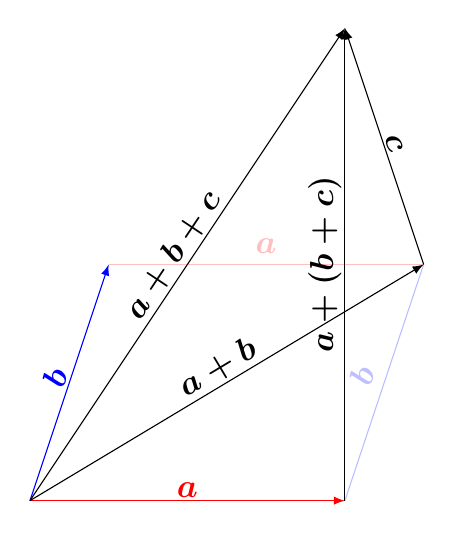
\begin{tikzpicture}[font=\boldmath]\large
    % Punkte
    \coordinate (A) at (0,0) {};
    \coordinate (B) at (4,0) {};
    \coordinate (C) at (1,3) {};
    \coordinate (D) at (5,3) {};
    \coordinate (E) at (4,6) {};

    % Draw the triangle
    \draw[blue!25]  (B) -- (D) node[sloped,midway,above] {$\vv{b}$};
    \draw[red!25]   (C) -- (D) node[sloped,midway,above] {$\vv{a}$};
    \draw[->,  red,   arrows={-latex}]  (A) -- (B) node[sloped,midway,above=-0.1cm] {$\vv{a}$};
    \draw[->,  blue,  arrows={-latex}]  (A) -- (C) node[sloped,midway,above=-0.1cm] {$\vv{b}$};
    \draw[->, black, arrows={-latex}]  (A) -- (D) node[sloped,midway,above=-0.1cm] {$ \vv{a} + \vv{b} $};
    \draw[->,  black,   arrows={-latex}]  (D) -- (E) node[sloped,midway,above=-0.1cm] {$\vv{c}$};
    \draw[->,  black,   arrows={-latex}]  (A) -- (E) node[sloped,midway,above=-0.1cm] {$\vv{a} + \vv{b} + \vv{c}$};
     \draw[->,  black,   arrows={-latex}]  (B) -- (E) node[sloped,midway,above=-0.1cm] {$\vv{a} + (\vv{b} + \vv{c})$};
\end{tikzpicture}
\end{center}
\end{satz}
\begin{b8d}{Besondere Vektoren}{}\index{Vektoren!Nullvektor}\index{Vektoren!Gegenvektor}
Bei der Rechnung mit Vektoren gibt es zwei besondere Vektoren zu betrachten. Hierbei handelt es sich um den sogenannten Nullvektor und den Gegenvektor.\\
Der Nullvektor $\vv{o}$ ist derjenige Vektor, der die Länge Null hat und bei dem sich bei er Addition mit anderen Vektoren nichts ändert. Es gilt: $$\vv{a} +\vv{o} = \vv{o} +\vv{a} = \vv{a}$$
Der Gegenvektor $-\vv{a}$ ist derjenige Vektor, der genauso lang wie der Vektor $\vv{a}$ ist allerdings entgegengerichtet. Für den Gegenvektor $-\vv{a}$ und den Vektor $\vv{a}$ gilt: $$\vv{a} +( -\vv{a} ) =\vv{a}-\vv{a}= \vv{o}$$
\end{b8d}
\begin{bem}{Vektorkette}{}\index{Vektoren!Vektorkette}
Werden mehrere Vektoren addiert so werden die jeweiligen Repräsentanten aneinandergereiht und das Ergebnis nennt man dann Vektorkette.
\end{bem}
\subsection{Vektor und Skalar}
\begin{merke}{Skalar}{}\index{Vektoren!Skalar}
   In der Analytischen Geometrie versteht man unter einem Skalar eine beliebige reelle Zahl. 
\end{merke}
\begin{defi}{Skalare Multiplikation}{}\index{Vektoren!Skalare Multiplikation}
Ein Vektor kann mit einer reellen Zahl durch eine Multiplikation verknüpft werden. Der Vektor $\lambda \cdot \vv{u}$ ist $|\lambda|$-mal so lang wie der Vektor $\vv{u}$. Dabei gilt für dis Zahl $\lambda$ folgendes $\lambda \in \mathds{R}$.\\
Für $\lambda > 0$ hat der Vektor $\lambda \cdot \vv{u}$ die gleiche Richtung wie der Vektor $\vv{u}$.\\
Für $\lambda < 0$ hat der Vektor $\lambda \cdot \vv{u}$ die entgegengesetzte Richtung wie der Vektor  $\vv{u}$.\\
\begin{center}
\begin{tikzpicture}[font=\boldmath]\large
    % Punkte
    \coordinate (A) at (0,0) {};
    \coordinate (B) at (2,1) {};
    \coordinate (C) at (6,2) {};
    \coordinate (D) at (2,0) {};
    \draw[->,  arrows={-latex}]  (A) -- (B) node[sloped,midway,above=-0.1cm] {$\vv{u}$};
    \draw[->,  arrows={-latex}]  (D) -- (C) node[sloped,midway,above=-0.1cm] {$2\cdot \vv{u}$};   
\end{tikzpicture}
\end{center}
\end{defi}
\begin{satz}{Rechenregeln für das Skalarprodukt}{}\index{Vektoren!Skalare Multiplikation}
Die Skalare Multiplikation folgt zwei Gesetzmäßigkeiten. dabei gilt $\lambda, \mu \in \mathds{R}$:
\begin{itemize}
    \item Assoziativgesetz: $\lambda \cdot \left(\mu \cdot \vv{u}\right) =\left( \mu \cdot \lambda \right)\vv{u}$
    \item Distributivgesetz 1: $\lambda \cdot \left(\vv{u} + \vv{v}\right) =\lambda \cdot \vv{u} + \lambda \cdot \vv{v} $
    \item Distributivgesetz 2: $\left( \lambda + \mu\right) \cdot \vv{u} =\lambda \cdot \vv{u} + \mu \cdot \vv{u}  $
\end{itemize}
\end{satz}
\begin{bem}{}{}
Beim aufstellen einer Vektorkette versucht man den Anfangs- und Endpunkt eines Vektors durch bekannte Vektoren zu verbinden. Der Vektor $\vv{AB}$ beginnt im Punkt $A$ und endet im Punkt $B$.

\end{bem}
\begin{bsp}{Vektorkette}{}
Die Vektoren $\vv{a}=\vv{AB}, \vv{b}=\vv{AD}$ und $\vv{c}=\vv{AS}$  spannen eine vierseitige Pyramide ABCDS auf, deren Grundfläche ein Parallelogramm ABCD ist. Der Fußpunkt der Pyramidenhöhe ist der Schnittpunkt der Diagonalen der Grundfläche.   
\begin{center}
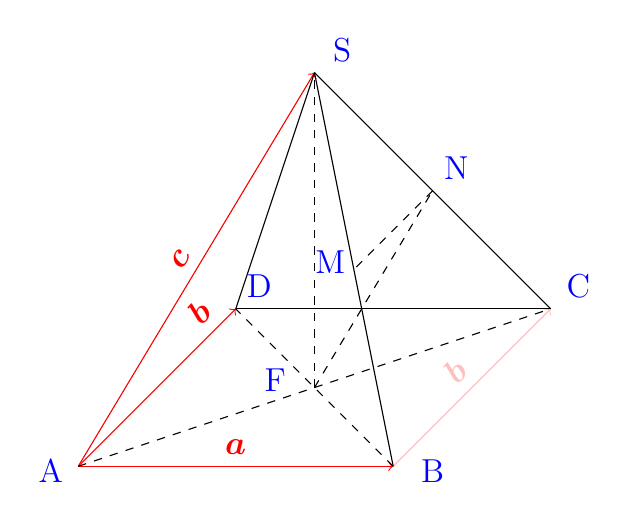
\begin{tikzpicture}[font=\boldmath]\large
    % Punkte
    \coordinate (A) at (0,0) {};
     \draw[blue] (-0.35,-0.35)   node [above] {A};
    \coordinate (B) at (4,0) {};
    \draw[blue] (4.5,-0.35)   node [above] {B};
    \coordinate (C) at (6,2) {};
    \draw[blue] (6.35,2)   node [above] {C};
    \coordinate (D) at (2,2) {};
    \draw[blue] (2.3,2)   node [above] {D};
    \coordinate (E) at (3,5) {};
    \draw[blue] (3.35,5)   node [above] {S};
    \coordinate (F) at (3,1) {};
    \draw[blue] (2.5,0.8)   node [above] {F};
    \coordinate (G) at (4.5,3.5) {};
    \draw[blue] (4.8,3.5)   node [above] {N};
    \coordinate (H) at (3.5,2.5) {};
    \draw[blue] (3.2,2.3)   node [above] {M};
    \draw[->, red]  (A) -- (B) node[sloped,midway,above] {$\vv{a}$};
    \draw[->,red!25]  (B) -- (C) node[sloped,midway,above] {$\vv{b}$};
    \draw  (C) -- (D) node[] {};
    \draw[->,red]  (A) -- (D) node[sloped,above,very near end] {$\vv{b}$};
   \draw[->,red]  (A) -- (E) node[sloped,midway,above] {$\vv{c}$};
   \draw  (E) -- (B) node[] {};
   \draw  (E) -- (C) node[] {};
   \draw  (E) -- (D) node[] {};
   \draw[dashed]  (A) -- (C) node[] {};
   \draw[dashed]  (B) -- (D) node[] {};
   \draw[dashed]  (F) -- (E) node[] {};
    \draw[dashed]  (G) -- (H) node[] {};
    \draw[dashed]  (F) -- (G) node[] {};
\end{tikzpicture}
\end{center}
Folgende Aufgaben sind typisch für Vektorketten
\begin{enumerate}
    \item Warum repräsentieren die Vektoren $\vv{BS}, \vv{CS}$ und $\vv{DS}$ \textcolor{red}{nicht} den Vektor $\vv{c}$?
    \begin{itemize}
        \item $\vv{BS}, \vv{CS}$ und $\vv{DS}$ sind gleich lang wie $\vv{c}$
        \item aber nicht \textcolor{red}{parallel} zu $\vv{c}$
    \end{itemize}
    \item Drücke die Vektoren $\vv{BS}, \vv{CS}, \vv{DS}$ und $\vv{AF}$ mithilfe der Vektoren $\vv{a}, \vv{b}$ und $\vv{
    c}$ aus.
    \begin{itemize}
        \item $\vv{BS}$
        \begin{itemize}
            \item[$\circ$] Um vom Startpunkt $B$ zum Endpunkt $S$ zu kommen, muss man von $B$ nach $A$ und dann nach $S$ \glqq laufen\grqq{}
            \item[$\circ$] $\vv{BS} = -\vv{a} + \vv{c} = \vv{c} - \vv{a}$
        \end{itemize}       
        \item $\vv{CS}$ 
        \begin{itemize}
            \item[$\circ$] Der Vektor $\vv{BC}$ ist ein Repräsentatnt des Vektors $\vv{b}$ 
            \item[$\circ$] $\vv{CS} = -\vv{b} - \vv{a} + \vv{c} = \vv{c} - \vv{a} -\vv{b}$
        \end{itemize}
        \item $\vv{DS}$ 
        \begin{itemize}
            \item[$\circ$] $\vv{DS} = -\vv{b} + \vv{c} = \vv{c} - \vv{b}$
        \end{itemize}
         \item $\vv{AF}$ 
         \begin{itemize}
             \item[$\circ$] Der Punkt $F$ liegt in der Mitte des Vektors $\vv{AC}$
             \item[$\circ$] $\vv{AC} = \vv{a} + \vv{b}$
             \item[$\circ$] $\vv{AF} = \dfrac{1}{2} \left(\vv{a} + \vv{b} \right)$
         \end{itemize}
    \end{itemize}
    \end{enumerate}
 In der Pyramide ist $M$ der Mittelpunkt der Seitenkante $\vv{BS}$ und $N$ der Mittelpunkt der Seitenkante  $\vv{CS}$.  
      \begin{enumerate}
        \item[3.] Drücke den Vektor $\vv{FN}$ mithilfe der Vektoren $\vv{a}, \vv{b}$ und $\vv{
    c}$ aus.
    \end{enumerate}
   \begin{multicols}{2}
    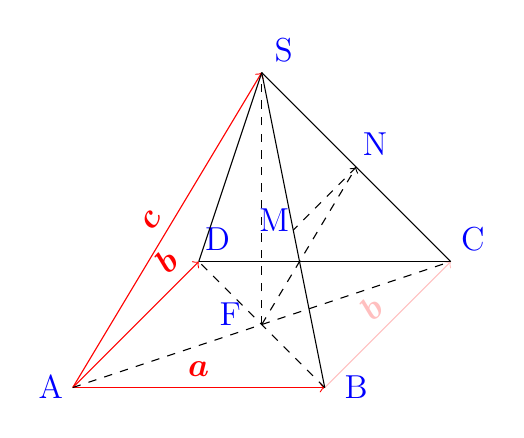
\begin{tikzpicture}[font=\boldmath, scale=0.8]\large
    % Punkte
    \coordinate (A) at (0,0) {};
     \draw[blue] (-0.35,-0.35)   node [above] {A};
    \coordinate (B) at (4,0) {};
    \draw[blue] (4.5,-0.35)   node [above] {B};
    \coordinate (C) at (6,2) {};
    \draw[blue] (6.35,2)   node [above] {C};
    \coordinate (D) at (2,2) {};
    \draw[blue] (2.3,2)   node [above] {D};
    \coordinate (E) at (3,5) {};
    \draw[blue] (3.35,5)   node [above] {S};
    \coordinate (F) at (3,1) {};
    \draw[blue] (2.5,0.8)   node [above] {F};
    \coordinate (G) at (4.5,3.5) {};
    \draw[blue] (4.8,3.5)   node [above] {N};
    \coordinate (H) at (3.5,2.5) {};
    \draw[blue] (3.2,2.3)   node [above] {M};
    \draw[->, red]  (A) -- (B) node[sloped,midway,above] {$\vv{a}$};
    \draw[->,red!25]  (B) -- (C) node[sloped,midway,above] {$\vv{b}$};
    \draw  (C) -- (D) node[] {};
    \draw[->,red]  (A) -- (D) node[sloped,above,very near end] {$\vv{b}$};
   \draw[->,red]  (A) -- (E) node[sloped,midway,above] {$\vv{c}$};
   \draw  (E) -- (B) node[] {};
   \draw  (E) -- (C) node[] {};
   \draw  (E) -- (D) node[] {};
   \draw[dashed]  (A) -- (C) node[] {};
   \draw[dashed]  (B) -- (D) node[] {};
   \draw[dashed]  (F) -- (E) node[] {};
    \draw[dashed]  (G) -- (H) node[] {};
    \draw[->,dashed]  (F) -- (G) node[] {};
\end{tikzpicture} 
    \begin{itemize}
        \item[$\circ$] Vektorkette von $F$ nach $C$ zu $N$.
     \begin{equation*}
            \begin{split}
                \vv{FN} &= \vv{FC} + \vv{CN}\\
                &=\vv{AF} + \dfrac{1}{2} \vv{CS}\\
                &= \dfrac{1}{2} \left(\vv{a} + \vv{b} \right) + \dfrac{1}{2}\left(\vv{c} - \vv{a} -\vv{b}\right)\\
                &=\dfrac{1}{2} \vv{a} + \dfrac{1}{2} \vv{b} + \dfrac{1}{2} \vv{c} - \dfrac{1}{2} \vv{a} -\dfrac{1}{2} \vv{b} \\
                &= \dfrac{1}{2}\vv{c}
            \end{split}
        \end{equation*}
        
    \end{itemize}
   \end{multicols}
   \begin{itemize}
       \item[$\circ$] Daraus folgt, dass der Vektor $\vv{FN}$ parallel und gleichgerichtet zum Vektor $\vv{c}$ aber nur halb so lang ist.
   \end{itemize}
   \begin{enumerate}
    \item[4.] Drücke den Vektor $\vv{MN}$ mithilfe der Vektoren $\vv{a}, \vv{b}$ und $\vv{
    c}$ aus.
    \begin{multicols}{2}
    \begin{itemize}
        \item[$\circ$] Vektorkette von $M$ über $B, C$ zum Punkt $N$.
     \begin{equation*}
            \begin{split}
                \vv{MN} &= - \dfrac{1}{2}\vv{BS} + \vv{BC} + \dfrac{1}{2} \vv{CS}\\
                &= -\dfrac{1}{2} \left( \vv{c} - \vv{a}\right) +\vv{b} + \dfrac{1}{2} \left(\vv{c} - \vv{a} -\vv{b}\right)\\
                &= -\dfrac{1}{2} \vv{c} +\dfrac{1}{2} \vv{a} +\vv{b} + \dfrac{1}{2} \vv{c} - \dfrac{1}{2}\vv{a} -\dfrac{1}{2}\vv{b}\\
                &= \dfrac{1}{2} \vv{b}
            \end{split}
        \end{equation*}  
        \item[$\circ$] Damit folgt, das die Mittellinie $MN$ parallel, gleichgerichtet aber nur halb so lang wie der Vektor $\vv{b}$ ist.
    \end{itemize}
    \end{multicols}
\end{enumerate}
\end{bsp}
\section{Der dreidimensionale Vektorraum}